% (c) 2012 - 2014 Dimitrios Vrettos - d.vrettos@gmail.com
% (c) 2014 Claudio Carboncini - claudio.carboncini@gmail.com
\chapter{Equazioni di primo grado}\label{cap:equazioni_I_grado}
\section{Identità ed equazioni}

Analizziamo le seguenti proposizioni:

\begin{enumeratea}
\item ``cinque è uguale alla differenza tra sette e due'';
\item ``la somma di quattro e due è uguale a otto'';
\item ``il doppio di un numero naturale è uguale alla differenza tra nove e il numero stesso'';
\item ``la somma di due numeri interi è uguale a dieci''.
\end{enumeratea}

Notiamo che sono tutte costruite con il predicato
``essere uguale a''. Riscriviamo in formula ciascuna di esse:
\begin{multicols}{4}
 \begin{enumeratea}
\item $5=7-2$;
\item $4+2=8$;
\item $2x=9-x$;
\item $x+y=10$.
\end{enumeratea}
\end{multicols}
Notiamo che le prime due contengono solamente numeri, le seconde
contengono anche variabili (lettere).

Le formule del primo tipo si dicono \emph{chiuse} e
di esse si può subito stabilire se sono vere o false; così in~$\insN$ la
formula~$5 = 7 - 2$ è vera, mentre~$4 + 2 = 8$ è falsa.

\begin{definizione}
 Le \emph{formule chiuse} costruite con il predicato
<<essere uguale>> si chiamano \emph{uguaglianze};
definito l'ambiente in cui vengono enunciate si può
immediatamente stabilire il loro valore di verità.
\end{definizione}

\begin{exrig}
 \begin{esempio}
 La formula chiusa~$1 - 6 = -5$ è un'uguaglianza
vera se la consideriamo nell'insieme~$\insZ$ degli interi
relativi, è falsa se la vediamo come sottrazione tra numeri naturali.
 \end{esempio}
\end{exrig}

Le formule c) e d) che contengono variabili si dicono \emph{aperte}; le variabili che compaiono sono chiamate
\emph{incognite}. Di tali formule non si può subito stabilire il valore di verità.

Quando alle incognite sostituiamo un numero, queste si trasformano in
formule chiuse e allora possiamo stabilirne il valore di verità
relativamente alla sostituzione effettuata.

\begin{exrig}
 \begin{esempio}
 Nella formula~$2x = 9 - x$ sostituiamo alla variabile~$x$ il valore $0$; quindi otteniamo:~$2\cdot 0=9-0 \Rightarrow~0=9$, falsa.

 Sostituiamo ora alla
variabile~$x$ il valore $3$; otteniamo~$2\cdot 3=9-3 \Rightarrow~6=6$, vera.
 \end{esempio}

 \begin{esempio}
 Nella formula~$x + y = 10$ sostituiamo
alle variabili coppie di numeri interi come~$x = 2$ e~$y = 5$; otteniamo~$2+5=10\Rightarrow~7= 10$, falsa. Se
sostituiamo~$x = 4$ e~$y = 6$ ci rendiamo subito conto che
l'uguaglianza ottenuta è vera. Esistono
molte altre coppie di numeri interi che rendono vera
l'uguaglianza.
 \end{esempio}
\end{exrig}

\begin{definizione}
 Le formule aperte costruite con il predicato essere uguale si chiamano
\emph{equazioni}; le due espressioni che compaiono a sinistra e a
destra del segno di uguaglianza si chiamano rispettivamente
\emph{primo membro} e \emph{secondo membro}.

L'insieme dei valori che sostituiti alle incognite trasformano l'equazione in
un'uguaglianza vera costituisce
l'\emph{insieme soluzione} ($\IS$) o più semplicemente la \emph{soluzione} dell'equazione.
\end{definizione}

Affronteremo per ora equazioni in
\emph{una sola incognita} che, dopo aver svolto eventuali calcoli nei due membri, comparirà a
\emph{grado} 1 e i cui \emph{coefficienti} sono \emph{numeri razionali}.
Cercheremo la sua soluzione
nell'insieme~$\insQ$ dei numeri razionali, salvo esplicita indicazione differente.
\begin{exrig}
 \begin{esempio}
Cercare le soluzioni nell'insieme indicato.
 \begin{enumeratea}
 \item $x^{2}=1 \text{ con }x\in\insN.$
Risulta vera solo se a~$x$ sostituiamo il valore~1; infatti~1 è
l'unico numero naturale il cui quadrato è~1.
L'insieme soluzione è~$\{1\}$.
 \item $x^{2}=1 \text{ con }x\in\insZ$.
Risulta vera se a
$x$ sostituiamo il valore~1 oppure il valore~$-1$; infatti sia~$-1$ che~1
elevati al quadrato danno~1. L'insieme soluzione è
$\{-1\text{,~}1\}$.
 \item $x^{2}+1=0\text{ con }x\in\insR$.
Essendo la formula a sinistra
dell'uguale la somma di un quadrato con il numero~1, si ottiene sempre
un numero~$\geq1$ e non si può ottenere $0$, pertanto è impossibile trovare una soluzione, ovvero l'insieme soluzione è $\emptyset$.
 \item $2x+3=(3+x)+x \text{ con } x\in\insQ$.
Eseguendo il semplice calcolo al secondo
membro, ci rendiamo conto che qualunque valore venga sostituito
all'incognita l'uguaglianza risulta
vera. L'insieme soluzione è~$\insQ$.
\end{enumeratea}
 \end{esempio}
\end{exrig}

In generale un'equazione in una incognita può essere:

\begin{enumeratea}
\item \emph{determinata}, quando l'insieme soluzione è un sottoinsieme proprio
dell'insieme numerico considerato;
\item \emph{impossibile}, quando l'insieme soluzione è l'insieme vuoto~$\emptyset$;
\item \emph{indeterminata} o \emph{identità}, quando l'insieme soluzione coincide con
l'insieme considerato.
\end{enumeratea}

\begin{exrig}
 \begin{esempio}
 Analizziamo le equazioni:
\begin{multicols}{3}
 \begin{enumeratea}
 \item $3\cdot x=0$;
 \item $0\cdot x=5$;
 \item $0\cdot x=0$.
\end{enumeratea}
\end{multicols}

Tutte e tre hanno la stessa struttura: il primo membro è il prodotto
di un coefficiente numerico per un valore incognito, il secondo membro
è un numero.

\begin{enumeratea}
 \item Per trovare l'insieme soluzione della prima equazione cerchiamo in~$\insQ$ il
numero che moltiplicato per~3 dà come prodotto~0. L'unico numero che rende vera
l'uguaglianza è zero. Quindi l'insieme delle soluzioni è~$\{0\}$. L'equazione è
\emph{determinata}.

 \item Per trovare l'insieme soluzione della seconda equazione cerchiamo in~$\insQ$ il
numero che moltiplicato per~0 dà come prodotto~5. Per la proprietà
della moltiplicazione quando moltiplichiamo per~0 il prodotto è~0,
non otterremo mai~5. Quindi l'insieme soluzione è
l'insieme vuoto $\emptyset$. L'equazione è
\emph{impossibile}.

 \item Per trovare l'insieme soluzione della terza equazione cerchiamo in~$\insQ$ il
numero che moltiplicato per zero dà come prodotto zero. Per la
proprietà della moltiplicazione quando moltiplichiamo per~0 il
prodotto è~0 qualunque sia l'altro fattore. Quindi
l'insieme delle soluzioni è~$\insQ$. L'equazione è
\emph{indeterminata}.
\end{enumeratea}
 \end{esempio}
\end{exrig}

%\subsection{Ricerca dell'insieme soluzione}
In alcuni casi la soluzione di un'equazione si può
trovare applicando semplicemente le proprietà delle operazioni.

\begin{exrig}
 \begin{esempio}
Analizziamo lo schema operativo dell'equazione~$3x-1=17 \text{ con } x\in\insN$.

Si opera sul valore incognito~$x$ per ottenere~17:

\[\text{\emph{entra} } x,\text{ si moltiplica per tre}\to~3\cdot x%
\text{ si sottrae } 1\to~3\cdot x-1 \text{ si ottiene } 17.\]

Qual è il valore in ingresso?

Per determinare il valore in ingresso basterà ripercorrere lo schema
 effettuando le operazioni inverse:
\[\text{\emph{da} } 17 \text{ aggiungi } 1\to~18 \text{ dividi per tre }\to~18:3 \to x.\]

La soluzione dell'equazione è~$x = 6$ e~$\IS$ (insieme
soluzione) è~$\{6\}$.
 \end{esempio}
\end{exrig}

\ovalbox{\risolvi \ref{ese:15.1}}\vspace{1.10ex}

Per risolvere un'equazione più complessa come
$\left(\dfrac{1}{2}x+3\right)\cdot (-5+x)=12x+\dfrac{1}{2}x^{2}$ con
$x\in~\insQ$, non possiamo applicare il procedimento precedente; potremmo
procedere per tentativi, sostituendo all'incognita
alcuni valori scelti a caso e verificando se il valore assunto dal
primo membro risulta uguale a quello assunto dal secondo membro. È
evidente però che questo procedimento raramente porterà a trovare
tutte le soluzioni di un'equazione.

\osservazione
Per risolvere un'equazione, cioè per determinare tutte
le eventuali soluzioni, si procede applicando i principi
d'equivalenza.

\section{Principi di equivalenza}

\begin{definizione}
 Due equazioni sono \emph{equivalenti} se hanno lo stesso insieme soluzione.
\end{definizione}

\begin{principio}[Primo principio di equivalenza]
 Aggiungendo o sottraendo ad ambo i membri di
un'equazione data uno stesso numero o una stessa
espressione (definita per ogni valore dell'incognita)
si ottiene un'equazione equivalente a quella data.
\end{principio}

\begin{principio}[Secondo principio di equivalenza]
 Moltiplicando o dividendo ambo i membri di
un'equazione per uno stesso numero non nullo o per
un'espressione non nulla (definita per ogni valore
attribuito all'incognita) si ottiene
un'equazione equivalente alla data.
\end{principio}


La forma più semplice (forma canonica) di un'equazione di primo grado in
un'incognita è del tipo:
\[x = \text{ numero}.\]

L'insieme soluzione di una
equazione di questo tipo è semplicemente:
\[\IS=\{\text{numero}\}.\]

Per esempio, l'insieme delle soluzioni dell'equazione
$x = -3$ è~$\IS =\{-3\}$.

I principi sopra enunciati permettono di trasformare qualunque equazione
nella forma canonica che ha lo stesso insieme soluzione di quella
assegnata.

\section{Equazioni intere}
In questo paragrafo vedremo come usare i principi
d'equivalenza prima enunciati per condurre
un'equazione alla forma canonica e dunque determinarne
la soluzione.

\begin{definizione}
\emph{Risolvere un'equazione} significa
determinare il suo Insieme Soluzione.
\end{definizione}

Cominciamo con alcuni esempi.

\begin{exrig}
 \begin{esempio}
Applicazione del~1{\textdegree} principio di equivalenza.

\begin{enumeratea}
\item $x-5=3$:
aggiungiamo~5 a entrambi i membri:~$x-5+5=3+5\:\Rightarrow\: x=8$, $\IS =\{8\}.$
\item $3x=2+2x$: sottraiamo~$2x$ a entrambi i membri:~$3x-2x=2+2x-2x\:\Rightarrow\: x=2$,
$\IS =\{2\}$.
\end{enumeratea}
 \end{esempio}

 \begin{esempio}
 Applicazione del~2{\textdegree} principio di equivalenza.

 \begin{enumeratea}
\item $3x=12$ dividiamo entrambi i membri per~3, si ha
\[\dfrac{3}{3}x=\dfrac{12}{3}\quad\Rightarrow\quad x=4\quad\to\quad\IS =\{4\}.\]
\item $\dfrac{1}{2}x=2$ moltiplichiamo entrambi i membri per~2, si ha
\[2\cdot {\dfrac{1}{2}}x=2\cdot 2\quad\Rightarrow\quad x=4\quad\to\quad\IS =\{4\}.\]
\end{enumeratea}
\end{esempio}

 \begin{esempio}
 $-2x+1=3x-5$.

\begin{enumeratea}
 \item Sottraiamo~1 a entrambi i membri~$-2x+1-1=3x-5-1$ quindi~$-2x=3x-6$;
\item sottraiamo~$3x$ a entrambi i membri~$-2x-3x=3x-3x-6$ quindi~$-5x=-6$;
\item dividiamo entrambi i membri per~$-5$:~$\dfrac{-5}{-5}x=\dfrac{-6}{-5}\quad\Rightarrow\quad x=\dfrac{6}{5}\quad\rightarrow\quad
\IS =\left\{\dfrac{6}{5}\right\}.$
\end{enumeratea}
 \end{esempio}

 \begin{esempio}
$(x+1)+3\cdot (2+x)=12x-1$.

\begin{enumeratea}
\item Svolgiamo i calcoli al primo e al secondo membro:~$x+1+6+3x=12x-1$;
\item sommiamo in ciascun membro i termini simili (se ce ne sono):~$4x+7=12x-1$;
\item sottraiamo ad ambo i membri il monomio~$12x$, applicando il primo principio:~$4x-12x+7=12x-1-12x$, sommiamo i
monomi simili al primo e al secondo membro e otteniamo~$-8x+7=-1$
\item sottraiamo ad ambo i membri il numero~7, applicando il primo principio e sommiamo i termini simili:
$-8x+7-7=-1-7\quad\Rightarrow\quad -8x=-8$;
\item dividiamo ambo i membri per~$-8$,
applicando il secondo principio:
$\dfrac{-8}{-8}x=\dfrac{-8}{-8}\quad\Rightarrow\quad x=1$.
\end{enumeratea}
L'equazione assegnata~$(x+1)+3\cdot (2+x)=12x-1$
risulta equivalente all'ultima trovata $x=1$, pertanto il
suo insieme soluzione è~$\IS = \{1\}$.
 \end{esempio}
\end{exrig}

\osservazione
La trasformazione di un'equazione nella forma canonica
prevede che il termine con l'incognita sia collocato da
una parte del segno uguale mentre dall'altra parte sia
posto il termine numerico.

Enunciamo alcune \emph{regole pratiche} che ci possono aiutare nella
procedura risolutiva e che discendono direttamente dal primo principio
d'equivalenza.
\begin{enumeratea}
\item Spostando da un membro all'altro un addendo occorre cambiargli il segno; l'equazione ottenuta è equivalente a quella data.

$2x-3=2$, per lasciare da sola la~$x$ al primo membro devo aggiungere~$+3$ al primo e
al secondo membro, ottengo~$2x-3+3=2+3$ da cui~$2x=2+3$.

L'effetto che si ha è che si è spostato il~$-3$ al
secondo membro cambiandolo di segno ($+3$).
\item Se in entrambi i membri dell'equazione compare uno
stesso addendo con lo stesso segno, esso può essere cancellato da
entrambi i membri: l'equazione che si ottiene è
equivalente a quella data.

Infatti:
$2x-3+x=2+x$. La~$x$ che sta al secondo membro va portata al primo, cambiandola di segno
$2x-3+x-x=2$ da cui~$2x-3=2$.

L'effetto che si ha è che si possono eliminare le due
$x$ che stanno una al primo membro e una al secondo membro.
\item Se il coefficiente dell'incognita è~$-1$, %ossia
l'equazione si presenta nella forma~$-x=n$, si
può cambiare di segno ai termini del primo e del secondo membro, per
ottenere la forma~$x=-n$ che è equivalente a quella data.

Cambiare di segno equivale a moltiplicare per
$-1$ i due membri dell'equazione.

Infatti:
$x-3=2x+1$. Dobbiamo portare~$2x$ al primo membro e~$-3$ al secondo membro, otteniamo
$x-2x=3+1$ da cui~$-x=4$.

Poiché il coefficiente della $x$ è negativo moltiplichiamo per~$-1$
primo e secondo membro
$-1\cdot (-x)=-1\cdot (4)$ da cui~$x=-4$.
\end{enumeratea}

\begin{exrig}
\begin{esempio}
 Risolvi l'equazione $5x+2\cdot (3-x)+1=-(4x-1)+2\cdot (6-x)$ applicando le regole pratiche sopra descritte.
\begin{enumeratea}
 \item svolgiamo i calcoli:~$5x+6-2x+1=-4x+1+12-2x$;
 \item eliminiamo i termini uguali che compaiono nei due membri:
 \[5x+6 \cancel{-2x}\cancel{+1}=-4x \cancel{+1}+12\cancel{-2x}\quad\Rightarrow\quad 5x+6=-4x+12;\]
 \item spostiamo il monomio~$-4x$ del secondo membro a sinistra del segno uguale e il numero~$+6$
da sinistra a destra, ottenendo:~$5x+4x=-6+12$;
\item sommando i termini simili nei due membri, otteniamo~$9x=+6$ da cui, dividendo per 9
 ambo i membri, si ottiene
 \[x=\dfrac{2}{3}\quad\to\quad \IS =\left\{\dfrac{2}{3}\right\}.\]
 \end{enumeratea}
\end{esempio}

\ovalbox{\risolvii \ref{ese:15.2}, \ref{ese:15.3}, \ref{ese:15.4}, \ref{ese:15.5}, \ref{ese:15.6}, \ref{ese:15.7}, \ref{ese:15.8}, \ref{ese:15.9}, \ref{ese:15.10}, \ref{ese:15.11}, \ref{ese:15.12}, \ref{ese:15.13},}

\vspace{1.10ex}
\ovalbox{\ref{ese:15.14}, \ref{ese:15.15}}

\subsection{Equazioni in cui l'incognita compare con grado maggiore di uno}
 \begin{esempio}

$(2x+1)\cdot (x-2)=2\cdot (x+1)^{2}-5x$.

Prima di iniziare la procedura risolutiva analizziamo i membri
dell'equazione: al primo membro compare il prodotto
di due polinomi di primo grado, nel secondo il quadrato di un binomio
di primo grado, pertanto l'incognita comparirà a grado due. Apparentemente
l'equazione è di secondo grado. Iniziamo la procedura
risolutiva:
\begin{enumeratea}
\item svolgiamo i calcoli e otteniamo:
\[2x^{2}-4x+x-2=2x^{2}+4x+2-5x\Rightarrow~2x^{2}-3x-2=2x^{2}-x+2;\]
\item applichiamo le regole pratiche eliminando i monomi
uguali con l'incognita al secondo grado e otteniamo
$-3x+x=+2+2$.
\end{enumeratea}

Abbiamo ottenuto un'equazione di primo grado; puoi
procedere da solo e determinare la forma canonica e l'$\IS$.

 \end{esempio}
\end{exrig}

\ovalbox{\risolvii \ref{ese:15.16}, \ref{ese:15.17}, \ref{ese:15.18}, \ref{ese:15.19}, \ref{ese:15.20}, \ref{ese:15.21}, \ref{ese:15.22}}

\subsection{Equazioni in cui l'incognita scompare}

\begin{exrig}\vspace{1.10ex}
 \begin{esempio}
 $\dfrac{4}{5}-\dfrac{x}{2}=\dfrac{2-5x}{10}$.

\begin{enumeratea}
\item Calcoliamo il~$\mcm$ tra i denominatori: in questo
caso~$\mcm(5\text{,~}2\text{,~}10) = 10$;

\item moltiplichiamo per~10 ambo i membri
dell'equazione:
$10\left(\dfrac{4}{5}-\dfrac{x}{2}\right)=10\left(\dfrac{2-5x}{10}\right)$;

\item eseguiamo i calcoli:~$8-5x=2-5x$;

\item applichiamo la regola pratica:
$-5x+5x=2-8$ i monomi in~$x$ si annullano!

\item sommando i monomi simili si ottiene:~$0\cdot x=-6$.
\end{enumeratea}

Il coefficiente dell'incognita è zero; non possiamo
applicare il secondo principio e dividere ambo i membri per zero.
D'altra parte non esiste nessun numero che moltiplicato
per zero dia come prodotto~$-6$. Quindi~$\IS =\emptyset $,
l'equazione risulta impossibile.
 \end{esempio}
\pagebreak
 \begin{esempio}
$\dfrac{x}{6}-\dfrac{2x}{3}=-{\dfrac{x}{2}}$.

\begin{enumeratea}
\item Calcoliamo il~$\mcm$ tra i denominatori: in questo
caso~$\mcm(6\text{,~}3\text{,~}2) = 6$.

\item moltiplichiamo per~6 ambo i membri
dell'equazione:
$6\left(\dfrac{x}{6}-\dfrac{2x}{3}\right)=6\left(-{\dfrac{x}{2}}\right)$;

\item eseguiamo i calcoli:~$x-4x=-3x$;

\item applicando il primo principio si ottiene~$0\cdot x=0$.

\end{enumeratea}

Il coefficiente dell'incognita è zero; non possiamo
applicare il secondo principio e dividere ambo i membri per zero.
D'altra parte per la proprietà della moltiplicazione
qualunque numero moltiplicato per zero dà come prodotto zero. Quindi
$\IS = \insQ$, l'equazione è indeterminata (identità).
 \end{esempio}
\end{exrig}

\section{Equazioni a coefficienti frazionari}
Vediamo, illustrando qualche esempio, come si procede.

\begin{exrig}
 \begin{esempio}
$\dfrac{2}{3}x+4-\dfrac{1}{2}+2x=\dfrac{x+2}{3}-\dfrac{5}{2}x+1$.

Sappiamo che il secondo principio d'equivalenza ci
permette di moltiplicare ambo i membri per uno stesso numero diverso da
zero per ottenere un'equazione equivalente alla data.
\begin{enumeratea}
\item Calcoliamo il~$\mcm$ tra i denominatori: in questo
caso~$\mcm(2\text{,~}3) = 6$;

\item moltiplichiamo per~6 ambo i membri
dell'equazione:
\[6\left(\dfrac{2}{3}x+4-\dfrac{1}{2}+2x\right)=6\left(\dfrac{x+2}{3}-\dfrac{5}{2}x+1\right);\]

\item eseguiamo i calcoli:~$4x+24-3+12x=2x+4-15x+6$.
\end{enumeratea}

I coefficienti dell'equazione sono ora numeri interi,
puoi procedere da solo come abbiamo visto negli esempi precedenti. Il risultato è $x=-\dfrac{11}{29}$.
\end{esempio}
\end{exrig}

\ovalbox{\risolvii \ref{ese:15.23}, \ref{ese:15.24}}\vspace{1.10ex}

%\subsection{Riassunto}
Riassumendo, quando si ha un'equazione del tipo~$A\cdot x=B$ con~$A$ e~$B$ numeri
razionali è la forma canonica dell'equazione di primo grado in una
incognita a coefficienti numerici.% è $A\cdot x=B$ con~$A$ e~$B$ numeri
%razionali.

Possono presentarsi i seguenti casi:
 \begin{itemize}
 \item se~$A\neq~0$ possiamo applicare il secondo principio
d'equivalenza dividendo ambo i membri per~$A$ quindi
$\IS =\left\{\dfrac{B}{A}\right\}$. L'equazione
è determinata.

 \item se~$A=0$ non possiamo applicare il secondo principio
d'equivalenza e dividere ambo i membri per~$A$ e si
presentano due casi:

\begin{itemize}
 \item $B=0$ allora~$\IS =\insQ$. L'equazione
è indeterminata.

\item $B\neq~0$ allora~$\IS =\emptyset $.
L'equazione è impossibile.
\end{itemize}
 \end{itemize}
%\pagebreak

Lo schema precedente si può rappresentare anche con un grafo ad
albero:
\begin{center}
 % (c) 2012 -2013 Dimitrios Vrettos - d.vrettos@gmail.com

\begin{tikzpicture}[x=5mm, y=5mm,font=\small]
\tikzstyle{level 1}=[level distance=2cm, sibling distance=2.5cm]
\tikzstyle{level 2}=[level distance=2cm, sibling distance=1.5cm]
\tikzstyle{point} = [circle,minimum width=3pt,fill, inner sep=0pt]

\node[point, label=left:{$A\cdot x =B$}] (aer) at (0,0) {}[grow'=right]
child {node[point, label=right:{$A\ne 0\to$ equazione determinata e $\IS=\left\{\dfrac{B}{A}\right\}$}] {} 
}
child {node[point, label=below:{$A=0$}] {} 
child {node[point,label=right:{$B=0\to$ equazione indeterminata e $\IS=\insQ$}] {}}
child {node[point,label=right:{$B\ne 0\to$ equazione impossibile e $\IS=\emptyset $}] {}}
} ;
\end{tikzpicture}
\end{center}

\ovalbox{\risolvii \ref{ese:15.25}, \ref{ese:15.26}, \ref{ese:15.27}, \ref{ese:15.28}, \ref{ese:15.29}, \ref{ese:15.30}, \ref{ese:15.31}, \ref{ese:15.32}, \ref{ese:15.33}, \ref{ese:15.34}, \ref{ese:15.35},}

\vspace{1.10ex}\ovalbox{\ref{ese:15.36}, \ref{ese:15.37}, \ref{ese:15.38}, \ref{ese:15.39}, \ref{ese:15.40}, \ref{ese:15.41}, \ref{ese:15.42}, \ref{ese:15.43}}
\newpage
% (c) 2012 Claudio Carboncini - claudio.carboncini@gmail.com
% (c) 2012 Dimitrios Vrettos - d.vrettos@gmail.com
\section{Esercizi}
\subsection{Esercizi dei singoli paragrafi}
\subsubsection*{\thechapter.1 - Cosa vuol dire scomporre in fattori}

\begin{esercizio}
\label{ese:15.1}
Associa le espressioni a sinistra con i polinomi a destra.
  \begin{multicols}{2}
\begin{enumeratea}
\item $(a+2b)^{2}$;
\item $3ab^{2}(a^{2}-b)$;
\item $(2a+3b)(a-2b)$;
\item $(3a-b)(3a+b)$;
\item $(a+b)^{3}$;
\item $(a+b+c)^{2}$;
\item $2a^{2}-4ab+3ab-6b^{2}$;
\item $a^{2}+4ab+4b^{2}$;
\item $9a^{2}-b^{2}$;
\item $3a^{3}b^{2}-3ab^{3}$;
\item $a^{2}+b^{2}+c^{2}+2ab+2bc+2ac$;
\item $a^{3}+3a^{2}b+3ab^{2}+b^{3}$.
\end{enumeratea}
  \end{multicols}
\end{esercizio}

\subsubsection*{\thechapter.2 - Raccoglimento totale a fattore comune}

\begin{esercizio}[\Ast]
\label{ese:15.2}
Scomponi in fattori raccogliendo a fattore comune.
\begin{multicols}{2}
\begin{enumeratea}
 \item $ax+3a^{2}x-abx$;
 \item $15b^{2}+12bc+21abx+6ab^{2}$;
 \item $15x^{2}y-10xy+25x^{2}y^{2}$.
\end{enumeratea}
\end{multicols}
\end{esercizio}

\begin{esercizio}[\Ast]
\label{ese:15.3}
Scomponi in fattori raccogliendo a fattore comune.
\begin{multicols}{2}
\begin{enumeratea}
 \item $-12a^{8}b^{9}-6a^{3}b^{3}-15a^{4}b^{3}$;
 \item $2ab^{2}+2b^{2}c-2a^{2}b^{2}-2b^{2}c^{2}$;
 \item $2m^{7}+8m^{6}+8m^{5}$.
\end{enumeratea}
\end{multicols}
\end{esercizio}

\begin{esercizio}[\Ast]
\label{ese:15.4}
Scomponi in fattori raccogliendo a fattore comune.
\begin{multicols}{3}
\begin{enumeratea}
 \item $9x^{2}b+6xb+18xb^{2}$;
 \item $20a^{5}+15a^{7}+10a^{4}$;
 \item $x^{2}b-x^{5}-4x^{3}b^{2}$.
\end{enumeratea}
\end{multicols}
\end{esercizio}

\begin{esercizio}
\label{ese:15.5}
Scomponi in fattori raccogliendo a fattore comune.
\begin{multicols}{3}
\begin{enumeratea}
 \item $3xy+6x^{2}$;
 \item $b^{3}+\dfrac{1}{3}b$;
 \item $3xy-12y^{2}$;
 \item $x^{3}-ax^{2}$;
 \item $9a^{3}-6a^{2}$;
 \item $5x^{2}-15x$.
\end{enumeratea}
\end{multicols}
\end{esercizio}

\begin{esercizio}
\label{ese:15.6}
Scomponi in fattori raccogliendo a fattore comune.
\begin{multicols}{3}
\begin{enumeratea}
 \item $18x^{2}y-12y^{2}$;
 \item $4x^{2}y-x^{2}$;
 \item $5x^{3}-2x^{2}$;
 \item $-2x^{3}+2x$;
 \item $3a+3$;
 \item $-8x^{2}y^{3}-10x^{3}y^{2}$.
\end{enumeratea}
\end{multicols}
\end{esercizio}

\begin{esercizio}
\label{ese:15.7}
Scomponi in fattori raccogliendo a fattore comune.
\begin{multicols}{2}
\begin{enumeratea}
 \item $\dfrac{2}{3}a^{2}b-\dfrac{4}{3}a^{4}b^{3}-\dfrac{5}{9}a^{2}b^{2}$;
 \item $12a^{3}x^{5}-18ax^{6}-6a^{3}x^{4}+3a^{2}x^{4}$;
 \item $\dfrac{2}{3}a^{4}bc^{2}-4ab^{3}c^{2}+\dfrac{10}{3}abc^{2}$;
 \item $-{\dfrac{3}{5}}a^{4}bx+\dfrac{3}{2}ab^{4}x-2a^{3}b^{2}x$.
\end{enumeratea}
\end{multicols}
\end{esercizio}

%\newpage
\begin{esercizio}
\label{ese:15.8}
Scomponi in fattori raccogliendo a fattore comune.
\begin{multicols}{2}
\begin{enumeratea}
 \item $-{\dfrac{5}{2}}a^{3}b^{3}-\dfrac{5}{3}a^{4}b^{2}+\dfrac{5}{6}a^{3}b^{4}$;
 \item $91m^{5}n^{3}+117m^{3}n^{4}$;
 \item $\dfrac{2}{3}a^{2}x+\dfrac{5}{4}ax^{2}-\dfrac{5}{4}ax$;
 \item $-5a^{2}+10ab^{2}-15a$.
\end{enumeratea}
\end{multicols}
\end{esercizio}

\begin{esercizio}
\label{ese:15.9}
Scomponi in fattori raccogliendo a fattore comune.
\begin{multicols}{3}
\begin{enumeratea}
 \item $ab^{2}-a+a^{2}$;
 \item $2b^{6}+4b^{4}-b^{9}$;
 \item $2a^{2}b^{2}x-4a^{2}b$;
 \item $-a^{4}-a^{3}-a^{5}$;
 \item $-3a^{2}b^{2}+6ab^{2}-15b$;
 \item $a^{2}b-b+b^{2}$.
\end{enumeratea}
\end{multicols}
\end{esercizio}

\begin{esercizio}
\label{ese:15.10}
Scomponi in fattori raccogliendo a fattore comune.
\begin{multicols}{3}
\begin{enumeratea}
 \item $2b^{6}+4b^{4}-b^{9}$;
 \item $-5a^{4}-10a^{2}-30a$;
 \item $-a^{2}b^{2}-a^{3}b^{5}+b^{3}$;
 \item $-2x^{6}+4x^{5}-6x^{3}y^{9}$;
 \item $-2x^{2}z^{3}+4z^{5}-6x^{3}z^{3}$;
 \item $-{\dfrac{4}{9}}x+\dfrac{2}{3}x^{2}-\dfrac{1}{3}x^{3}$.
\end{enumeratea}
\end{multicols}
\end{esercizio}

\begin{esercizio}
\label{ese:15.11}
Scomponi in fattori raccogliendo a fattore comune.
\begin{multicols}{2}
\begin{enumeratea}
 \item $\dfrac{1}{2}a^{2}+\dfrac{1}{2}a$;
 \item $a^{n}+a^{n-1}+a^{n-2}$;
 \item $\dfrac{1}{3}ab^{3}+\dfrac{1}{6}a^{3}b^{2}$;
 \item $a^{n}+a^{2n}+a^{3n}$.
\end{enumeratea}
\end{multicols}
\end{esercizio}

\begin{esercizio}
\label{ese:15.12}
Scomponi in fattori raccogliendo a fattore comune.
\begin{multicols}{2}
\begin{enumeratea}
 \item $2x^{2n}-6x^{(n-1)}+4x^{(3n+1)}$;
 \item $a^{2}x^{n-1}-2a^{3}x^{n+1}+a^{4}x^{2n}$;
 \item $a(x+y)-b(x+y)$;
 \item $(x+y)^{3}-(x+y)^{2}$.
\end{enumeratea}
\end{multicols}
\end{esercizio}

\begin{esercizio}[\Ast]
\label{ese:15.13}
Scomponi in fattori raccogliendo a fattore comune.
 \begin{multicols}{2}
 \begin{enumeratea}
 \item $a^{n}+a^{n+1}+a^{n+2}$;
 \item $(a+2)^{3}-(a+2)^{2}-a-2$;
 \item $2a(x-2)+3x(x-2)^{2}-(x-2)^{2}$.
\end{enumeratea}
 \end{multicols}
\end{esercizio}

\begin{esercizio}[\Ast]
Scomponi in fattori raccogliendo a fattore comune.
\label{ese:15.14}
 \begin{multicols}{2}
 \begin{enumeratea}
 \item $x^{2}(a+b)^{3}+x^{3}(a+b)+x^{5}(a+b)^{2}$;
 \item $3(x+y)^{2}-6(x+y)+2x(x+y)$.
\end{enumeratea}
 \end{multicols}
\end{esercizio}

\begin{esercizio}
\label{ese:15.15}
Scomponi in fattori raccogliendo a fattore comune.
\begin{multicols}{2}
\begin{enumeratea}
 \item $5y^{3}(x-y)^{3}-3y^{2}(x-y)$;
 \item $5a(x+3y)-3(x+3y)$;
 \item $2x(x-1)-3a^{2}(x-1)$;
 \item $2(x-3y)-y(3y-x)$.
\end{enumeratea}
\end{multicols}
\end{esercizio}

\begin{esercizio}[\Ast]
Scomponi in fattori raccogliendo a fattore comune.
\label{ese:15.16}
\begin{multicols}{2}
 \begin{enumeratea}
 \item $3x^{2}(a+b)-2x^{3}(a+b)+5x^{5}(a+b)$;
 \item $(2x-y)^{2}-5x^{3}(2x-y)-3y(2x-y)^{3}$.
\end{enumeratea}
\end{multicols}
\end{esercizio}
%\newpage
\subsubsection*{\thechapter.3 - Raccoglimento parziale a fattore comune}

\begin{esercizio}[\Ast]
\label{ese:15.17}
Scomponi in fattori con il raccoglimento parziale a fattore comune, se possibile.
\begin{multicols}{3}
 \begin{enumeratea}
 \item $2x-2y+ax-ay$;
 \item $3ax-6a+x-2$;
 \item $ax+bx-ay-by$.
\end{enumeratea}
\end{multicols}
\end{esercizio}

\begin{esercizio}
\label{ese:15.18}
Scomponi in fattori con il raccoglimento parziale a fattore comune, se possibile.
\begin{multicols}{2}
\begin{enumeratea}
 \item $3ax-9a-x+3$;
 \item $ax^{3}+ax^{2}+bx+b$;
 \item $2ax-4a-x+2$;
 \item $b^{2}x+b^{2}y+2ax+2ay$.
\end{enumeratea}
\end{multicols}
\end{esercizio}

\begin{esercizio}[\Ast]
\label{ese:15.19}
Scomponi in fattori con il raccoglimento parziale a fattore comune, se possibile.
\begin{multicols}{3}
 \begin{enumeratea}
 \item $3x^{3}-3x^{2}+3x-3$;
 \item $x^{3}-x^{2}+x-1$;
 \item $ay+2x^{3}-2ax^{3}-y$.
\end{enumeratea}
\end{multicols}
\end{esercizio}

\begin{esercizio}
\label{ese:15.20}
Scomponi in fattori con il raccoglimento parziale a fattore comune, se possibile.
\begin{multicols}{2}
\begin{enumeratea}
 \item $-x^{3}+x^{2}+x-1$;
 \item $x^{3}+x^{2}-x-1$;
 \item $x^{3}-1-x+x^{2}$;
 \item $-x^{3}-x-1-x^{2}$.
\end{enumeratea}
\end{multicols}
\end{esercizio}

\begin{esercizio}
\label{ese:15.21}
Scomponi in fattori con il raccoglimento parziale a fattore comune, se possibile.
\begin{multicols}{2}
\begin{enumeratea}
 \item $x^{3}+x^{2}+x+1$;
 \item $b^{2}x-b^{2}y+2x-2y$;
 \item $b^{2}x-b^{2}y-2ax-2ay$;
 \item $xy+x+ay+a+by+b$.
\end{enumeratea}
\end{multicols}
\end{esercizio}

\begin{esercizio}
\label{ese:15.22}
Scomponi in fattori con il raccoglimento parziale a fattore comune, se possibile.
\begin{multicols}{2}
\begin{enumeratea}
 \item $3x+6+ax+2a+bx+2b$;
 \item $2x-2+bx-b+ax-a$;
 \item $2x-2+bx-b-ax+a$;
 \item $2x+2+bx-b-ax+a$.
\end{enumeratea}
\end{multicols}
\end{esercizio}

\begin{esercizio}
\label{ese:15.23}
Scomponi in fattori con il raccoglimento parziale a fattore comune, se possibile.
\begin{multicols}{2}
\begin{enumeratea}
 \item $2x-b+ax-a-2+bx$;
 \item $a^{3}+2a^{2}+a+2$;
 \item $a^{2}x+ax-a-1$;
 \item $3xy^{3}-6xy-ay^{2}+2a$.
\end{enumeratea}
\end{multicols}
\end{esercizio}

\begin{esercizio}
\label{ese:15.24}
Scomponi in fattori con il raccoglimento parziale a fattore comune, se possibile.
\begin{multicols}{2}
\begin{enumeratea}
 \item $a^{2}x^{3}+a^{2}x^{2}+a^{2}x-2x^{2}-2x-2$;
 \item $3x^{4}-3x^{3}+3x^{2}-3x$;
 \item $2ax-2a+abx-ab+a^{2}x-a^{2}$;
 \item $3x^{4}y^{4}-6x^{4}y^{2}-ax^{3}y^{3}+2ax^{3}y$.
\end{enumeratea}
\end{multicols}
\end{esercizio}

\begin{esercizio}
\label{ese:15.25}
Scomponi in fattori con il raccoglimento parziale a fattore comune, se possibile.
\begin{multicols}{2}
\begin{enumeratea}
 \item $b^{2}x-2bx+by-2y$;
 \item $\dfrac{2}{3}x^{3}-\dfrac{1}{3}x^{2}+2x-1$;
 \item $ax+bx+2x-a-b-2$;
 \item $3(x+y)^{2}+5x+5y$.
\end{enumeratea}
\end{multicols}
\end{esercizio}

%\newpage
\begin{esercizio}[\Ast]
\label{ese:15.26}
Scomponi in fattori con il raccoglimento parziale a fattore comune, se possibile.
\begin{multicols}{2}
\begin{enumeratea}
 \item $bx^{2}-bx+b+x^{2}-x+1$;
 \item $a^{3}-a^{2}b^{2}-ab+b^{3}$;
 \item $\dfrac{1}{5}a^{2}b+3ab^{2}-\dfrac{1}{3}a-5b$.
\end{enumeratea}
\end{multicols}
\end{esercizio}

\begin{esercizio}
\label{ese:15.27}
Scomponi in fattori con il raccoglimento parziale a fattore comune, se possibile.
\begin{multicols}{2}
\begin{enumeratea}
 \item $3x^{4}+9x^{2}-6x^{3}-18x$;
 \item $2a-a^{2}+8b-4ab$;
 \item $4x^{2}+3a+4xy-4ax-3y-3x$;
 \item $3x^{4}-3x^{3}+2x-2$.
\end{enumeratea}
\end{multicols}
\end{esercizio}

\begin{esercizio}[\Ast]
\label{ese:15.28}
Scomponi in fattori con il raccoglimento parziale a fattore comune, se possibile.
\begin{multicols}{2}
 \begin{enumeratea}
 \item $(a-2)(a-3)+ab-2b$;
 \item $\dfrac{1}{8}x^{3}-2xy^{2}+\dfrac{1}{2}yx^{2}-8y^{3}$;
 \item $ab-bx^{2}-\dfrac{2}{3}ax+\dfrac{2}{3}x^{3}$.
\end{enumeratea}
\end{multicols}
\end{esercizio}

\begin{esercizio}[\Ast]
\label{ese:15.29}
Scomponi in fattori con il raccoglimento parziale a fattore comune, se possibile.
\begin{enumeratea}
 \item $45x^{3}+15xy+75x^{2}y+21x^{2}y^{2}+7y^{3}+35xy^{3}$;
 \item $10x^3-12x^2-5xy+6y$;
 \item $6a^3+3a^2b-2ab^3-b^4$.
\end{enumeratea}
\end{esercizio}

\begin{esercizio}[\Ast]
\label{ese:15.30}
Scomponi in fattori raccogliendo prima a fattore comune totale e poi parziale.
\begin{multicols}{2}
 \begin{enumeratea}
 \item $a^{14}+4a^{10}-2a^{12}-8a^{8}$;
 \item $3x^{2}(x+y)^{2}+5x^{3}+5x^{2}y$;
 \item $ax^{3}y+ax^{2}y+axy+ay$.
\end{enumeratea}
\end{multicols}
\end{esercizio}

\begin{esercizio}
\label{ese:15.31}
Scomponi in fattori raccogliendo prima a fattore comune totale e poi parziale.
\begin{multicols}{2}
\begin{enumeratea}
 \item $b^{2}x+b^{2}y-2bx-2by$; %ex63
 \item $b^{2}x-2bx-2by+b^{2}y$;%ex65
 \item $2ab^{2}+2b^{2}c-2a^{2}b^{2}-2ab^{2}c$; %ex67
 \item $3ax+6a+a^{2}x+2a^{2}+abx+2ab$.%ex69
\end{enumeratea}
\end{multicols}
\end{esercizio}

\begin{esercizio}[\Ast]
\label{ese:15.32}
Scomponi in fattori raccogliendo prima a fattore comune totale e poi parziale.
\begin{enumeratea}
 \item $2^{11}x^{2}+2^{12}x+2^{15}x+2^{16}$;
 \item $6x^{2}+6xy-3x(x+y)-9x^{2}(x+y)^{2}$;
 \item $2x^{3}+2x^{2}-2ax^{2}-2ax$.

\end{enumeratea}
\end{esercizio}

\begin{esercizio}
\label{ese:15.33}
Scomponi in fattori raccogliendo prima a fattore comune totale e poi parziale.
\begin{multicols}{2}
\begin{enumeratea}
 \item $2bx^{2}+4bx-2x^{2}-4ax$;
 \item $x^{4}+x^{3}-x^{2}-x$;
 \item $15x(x+y)^{2}+5x^{2}+5xy$;
 \item $2a^{2}mx-2ma^{2}-2a^{2}x+2a^{2}$.
\end{enumeratea}
\end{multicols}
\end{esercizio}

\begin{esercizio}[\Ast]
\label{ese:15.34}
Scomponi in fattori raccogliendo prima a fattore comune totale e poi parziale.
\begin{enumeratea}
 \item $\dfrac{2}{3}ax^{3}-\dfrac{1}{3}ax^{2}+\dfrac{2}{3}ax-\dfrac{1}{3}a$;
 \item $\dfrac{7}{3}x^{2}-\dfrac{7}{3}xy+\dfrac{1}{9}x^{3}-\dfrac{1}{9}x^{2}y-\dfrac{5}{9}(x^{2}-xy)$;
 \item $2b(x+1)^{2}-2bax-2ba+4bx+4b$.
\end{enumeratea}
\end{esercizio}

\subsection{Risposte}

\paragraph{\thechapter.2}
a)~$ax(3a-b+1)$,\quad b)~$3b(7ax+2ab+5b+4c)$, \quad c)~$5xy(5xy+3x-2)$.

\paragraph{\thechapter.3}
a)~$-3a^{3}b^{3}\left(4a^{5}b^{6}+5a+2\right)$,\quad b)~$2b^{2}(a+c-a^{2}-c^{2})$, \quad c)~$2m^{5}\left(m+2\right)^{2}$.

\paragraph{\thechapter.4}
a)~$3bx(3x+6b+2)$,\quad b)~$5a^{4}\left(3a^{3}+4a+2\right)$, \quad c)~$-x^{2}\left(x^{3}+4b^{2}x-b\right)$.

\paragraph{\thechapter.13}
a)~$a^{n}(1+a+a^{2})$,\quad b)~$(a+2)\left(a^{2}+3a+1\right)$, \quad c)~$(x-2)\left(3x^2-7x+2a+2\right)$.

\paragraph{\thechapter.14}
a)~$x^{2}(a+b)(ax^{3}+bx^{3}+x+a^{2}+2ab+b^{2})$,\quad b)~$(x+y)\left(5x+3y-6\right)$.

\paragraph{\thechapter.16}
a)~$x^{2}(a+b)(5x^{3}-2x+3)$,\quad b)~$(2x-y)\left(2x-y-5x^3-12x^2y+12xy^2-3y^3\right)$.

\paragraph{\thechapter.17}
a)~$(x-y)(2+a)$,\quad b)~$(x-2)(3a+1)$, \quad c)~$(a+b)(x-y)$.

\paragraph{\thechapter.19}
a)~$(3x-3)\left(x^2+1\right)$,\quad b)~$(x-1)\left(x^{2}+1\right)$, \quad c)~$(a-1)\left(y-2x^{3}\right)$.

\paragraph{\thechapter.26}
a)~$(b+1)(x^{2}-x+1)$,\quad b)~$\left(a^{2}-b\right)\left(a-b^{2}\right)$, \quad c)~$\left(\frac{3}{5}ab-1\right)\left(\frac{1}{3}a+5b\right)$.

\paragraph{\thechapter.28}
a)~$(a-2)(a-3+b)$,\quad b)~$(x+4y)\left(\frac{1}{8}x^2-2y^2\right)$, \quad c)~$\left(a-x^2\right)\left(b-\frac{2}{3}x\right)$.

\paragraph{\thechapter.29}
a)~$\left(15x+7y^{2}\right)\left(3x^{2}+y+5xy\right)$,\quad b)~$\left(2x^2-y\right)(5x-6)$, \quad c)~$(3a^2-b^3)(2a+b)$.

\paragraph{\thechapter.30}
a)~$a^{8}\left(a^{2}-2\right)\left(a^{4}+4\right)$,\quad b)~$x^{2}(x+y)(3x+3y+5)$, \quad c)~$ay(x+1)(x^{2}+1)$.

\paragraph{\thechapter.32}
a)~$2^{11}(x+2)(x+16)$,\quad b)~$-3x(x+y)\left(3x^2+3xy-1\right)$, \quad c)~$2x(x+1)(x-a)$.

\paragraph{\thechapter.34}
a)~$\frac{1}{3}a(x^{2}+1)(2x-1)$,\quad b)~$\frac{1}{9}x(x-y)(16+x)$, \quad c)~$2b(x+1)(x-a+3)$.

\cleardoublepage
